\documentclass[10pt]{exam}
\usepackage[hon]{template-for-exam}
\usepackage{graphicx}
\usepackage{tikz}
\usetikzlibrary{patterns,shapes.geometric}

\title{Golden Egg Lab}
\author{Rohrbach}
\date{\today}

\begin{document}
\maketitle



\section*{Previously on the island...}

Recall, the Sink the Boat story from last semester.  You had defeated the enemy that came to your secluded island to steal your peace and quiet.


\section*{The Problem}

After defeating your enemeny, you lived happily for a few more years. Suddenly, you started missing your previous civilized life with all its gadgets (internet, games, cell phones, etc.) and you decided to return home. In the meantime, you have discovered a mine with ``golden eggs'' (marbles) and you want to take some home to ensure a pleasant retirement. You will use the natural ``hills'' of your island (tracks) to roll the ``golden eggs'' into a boat near the shore of the island. 

\vspace{2em}

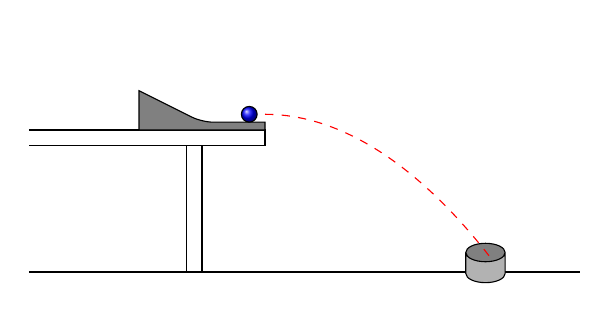
\begin{tikzpicture}
  \draw[thick] (0,0) -- (7,0);
  \draw (0,1.8)
    -- ++ (3,0)
    -- ++ (0,-.2)
    -- ++ (-3,0);
  \draw (2,0) rectangle (2.2,1.6);
  \draw[fill=gray] (3,1.9)
    -- ++(0,-.1)
    -- ++(-1.6,0) 
    -- ++(0,0.5)
    to[rounded corners] ++(.8,-.4)
    -- cycle;
  \draw[shading=ball] (2.8,2) circle (0.1);
  \node[
    cylinder, 
    draw=black, 
    shape border rotate=90,
    minimum size=0.5cm,
    cylinder uses custom fill,
    cylinder body fill = gray!60,
    cylinder end fill = gray,
    anchor=center
    ] at (5.8,0) {};
  \clip (0,0.2) rectangle (7,3.1);
  \draw[dashed,red] (3,2) parabola (6,0);
\end{tikzpicture}

\vspace{2em}

\noindent
Decide where to place your boat so that a Golden Egg rolled from the top of the hill lands in your boat.


\section*{Your Solution}

Initially, you should use the whiteboard to work out the problem with your group.  When you're ready, include a diagram of the setup and show your work below (or on a separate sheet of paper).  You will be taking a picture of your work and then explaining it in your lab report.

\pagebreak


\section*{Lab Report Guidelines}

\subsection*{Purpose:}  
Write a brief statement explaining the problem.  What are you trying to accomplish?


\subsection*{Procedure/Calculations:}
Take a picture with your phone of your calculations and insert them in the word document.  Your calculations should be \emph{well organized} and should include a labeled \emph{diagram} of the lab setup.  You should also include a paragraph explaining the mathematical steps you used to solve the problem 

\subsection*{Results:}
Write a few sentences explaining your results.  Did you achieve the objective?  Was there any obvious issues in completing the launch?

\subsection*{Conclusion/Discussion:}
Write a paragraph that addresses the following questions.

\begin{enumerate}
  \item Explain your results. Were you accurate?  Why or why not? 
  \item Explain where the errors came from.  Be specific—you should never use vague allusions to ``human error.''  What could be done in the future to improve your results?
  \item What could be done in the future to improve your results
\end{enumerate}
	


\end{document}